\section{Databases for the Generic T-tail Transport Aircraft} \label{sec:gtt_dbs}

Thus far, the examples of probabilistic databases has been focused on the baseline aerodynamics of the aircrafts in question. 
This section will focus on controls databases which define the aircraft's response to a control surface deflection by providing the resulting rotational moments that are imparted. 
As mentioned in Section \ref{subsec:gtt_cfd_data_gen}, the difficulty in modeling control surface deflections precludes the use of CFD simulation data in building these controls databases. 
Consequently, these databases can be, at most, two-fidelity ones with AVL simulations and wind tunnel experiments as the data sources. 
A number of visualizations of the GP regressions are presented in this section.
To showcase certain advantages of using multi-fidelity data, single-fidelity GP results using AVL data and WT data in isolation are presented.
This is contrasted with the two-fidelity GP results that use both sets of data. 

In the interest of brevity and since the maneuver of interest focuses on the roll-authority of the aircraft, these visualizations will present the roll moment imparted due to aileron deflection ($C_{l{\delta_a}}$).
This is just one of the 18 coefficients (Table \ref{tab:control_db}) that define the aircraft's control behavior, but is the most pivotal for the maneuver of interest. 

\subsection{Single-fidelity databases}
The results of the single-fidelity GP regression performed on AVL data and wind tunnel data are presented in Figures \ref{fig:gtt_avl_ctrl_gps} and \ref{fig:gtt_wt_ctrl_gps} respectively. 
With controls databases, a new input variable defining the control surface deflection angle ($\delta_*$) is used in addition to $\alpha$ and $\beta$ .
This makes visualizing the results of 3-dimensional GP in 3D space challenging. 
For both figures, a set of 4 surfaces or lines are shown in the first three subfigures. 
Each individual line or surface corresponds to a particular aileron deflection angle.
They are stacked in order of increasing deflection angle, where the angles are $\delta_a \in \{-25^\circ, -10^\circ, 10^\circ, 25^\circ\}$


\begin{figure}
    \centering
    \begin{subfigure}[\label{subfig:gtt_avl_ctrl_surf}3-Dimensional function in $\alpha$, $\beta$, and $\delta_a$] {
        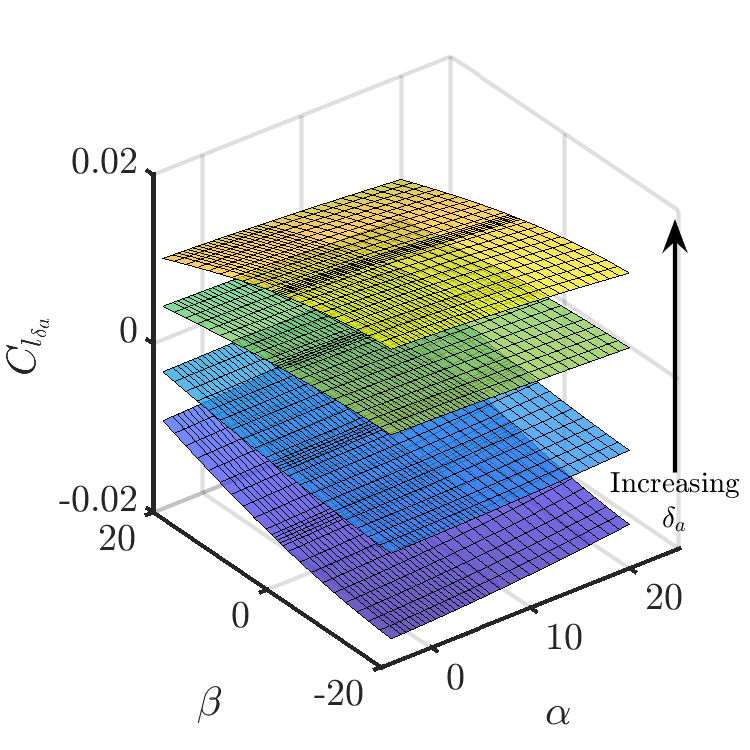
\includegraphics[trim=0 0 0 0, clip, width=.48\textwidth]{code/image_gen/gmatt/1f/avl/images/gps/CRMAIL.png} }
    \end{subfigure}
    \hfill
    \begin{subfigure}[\label{subfig:gtt_avl_ctrl_beta}Variation in $\beta$ at $\alpha=8^\circ$]{
        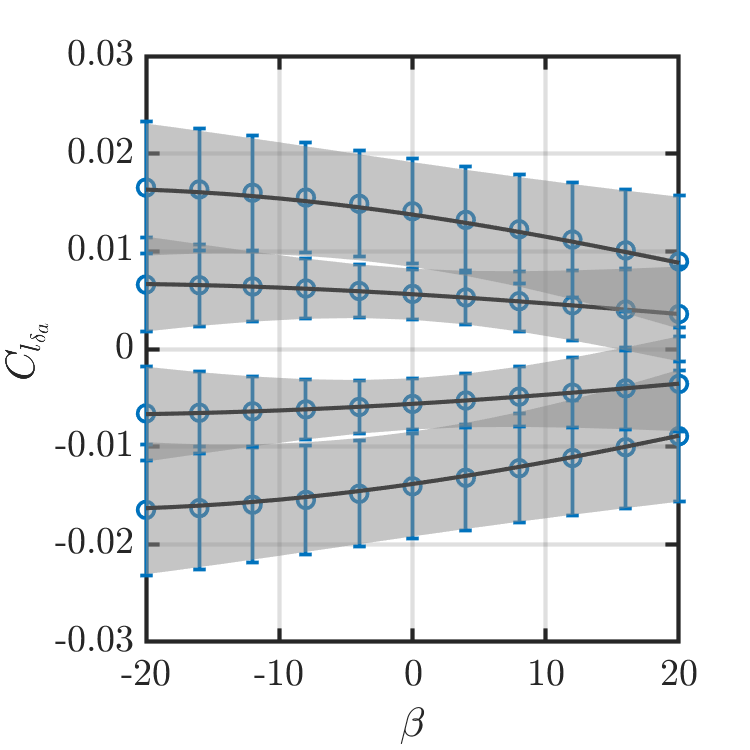
\includegraphics[trim=0 0 0 0, clip, width=.48\textwidth]{code/image_gen/gmatt/1f/avl/images/gps/CRMAIL_alpha=8.png}
    }
    \end{subfigure}
    \hfill
    \begin{subfigure}[\label{subfig:gtt_avl_ctrl_alpha}Variation in $\alpha$ at $\beta=4^\circ$]{
        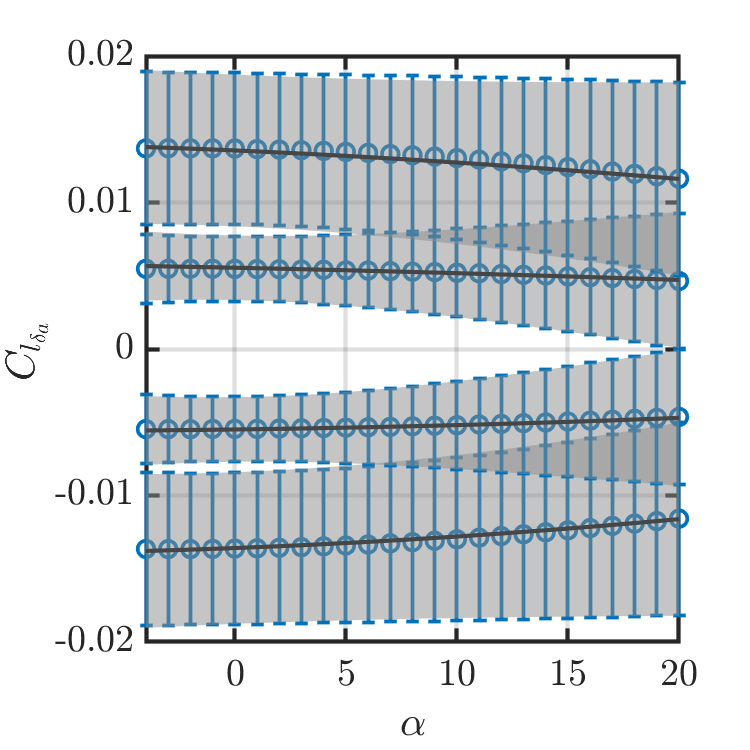
\includegraphics[trim=0 0 0 0, clip, width=.48\textwidth]{code/image_gen/gmatt/1f/avl/images/gps/CRMAIL_beta=4.png} 
    }
    \end{subfigure}
    \hfill
    \begin{subfigure}[\label{subfig:gtt_avl_ctrl_defl}Variation in $\delta_a$ at $\alpha = 8^\circ$ and $\beta=4^\circ$]{
        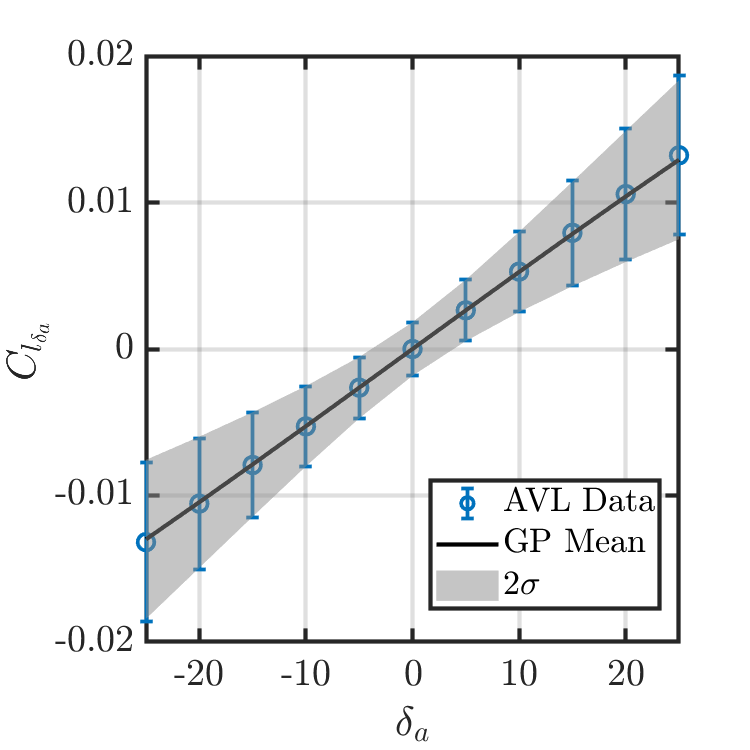
\includegraphics[trim=0 0 0 0, clip, width=.48\textwidth]{code/image_gen/gmatt/1f/avl/images/gps/CRMAIL_alpha=8_beta=4.png} 
    }
    \end{subfigure}
    \caption{Visualization of the 3-Dimensional AVL data and resulting single-fidelity GP for the rolling moment due to aileron deflections. \label{fig:gtt_avl_ctrl_gps}}
\end{figure}

\begin{figure}
    \centering
    \begin{subfigure}[\label{subfig:gtt_wt_ctrl_surf}3-Dimensional function in $\alpha$, $\beta$, and $\delta_a$] {
        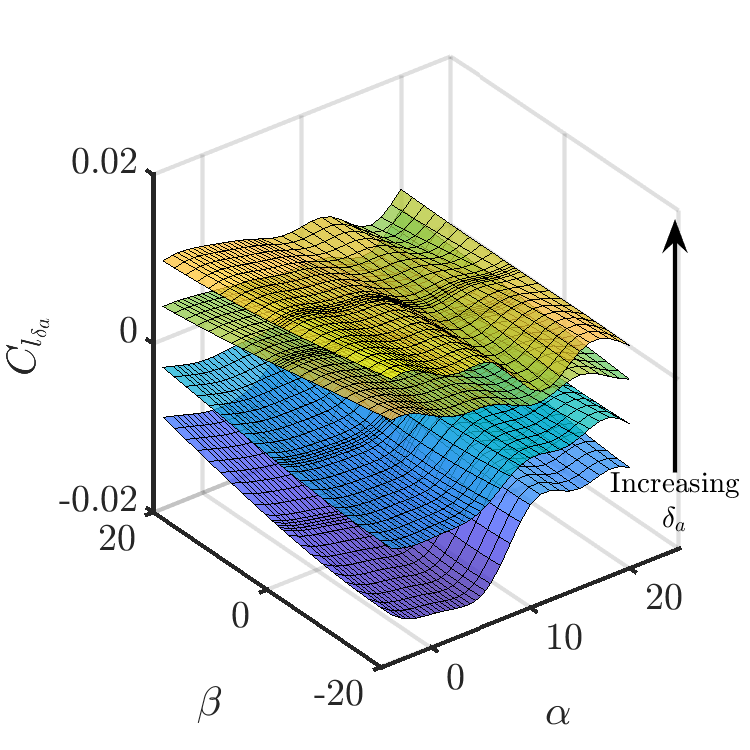
\includegraphics[trim=0 0 0 0, clip, width=.48\textwidth]{code/image_gen/gmatt/1f/wt/images/gps/CRMAIL.png} }
    \end{subfigure}
    \hfill
    \begin{subfigure}[\label{subfig:gtt_wt_ctrl_beta}Variation in $\beta$ at $\alpha=8^\circ$]{
        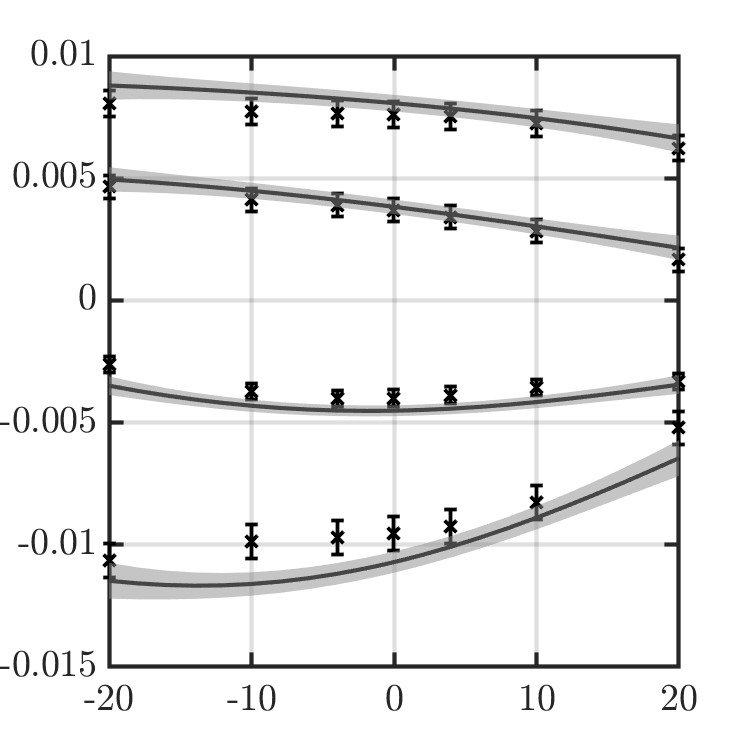
\includegraphics[trim=0 0 0 0, clip, width=.48\textwidth]{code/image_gen/gmatt/1f/wt/images/gps/CRMAIL_alpha=8.png}
    }
    \end{subfigure}
    \hfill
    \begin{subfigure}[\label{subfig:gtt_wt_ctrl_alpha}Variation in $\alpha$ at $\beta=4^\circ$]{
        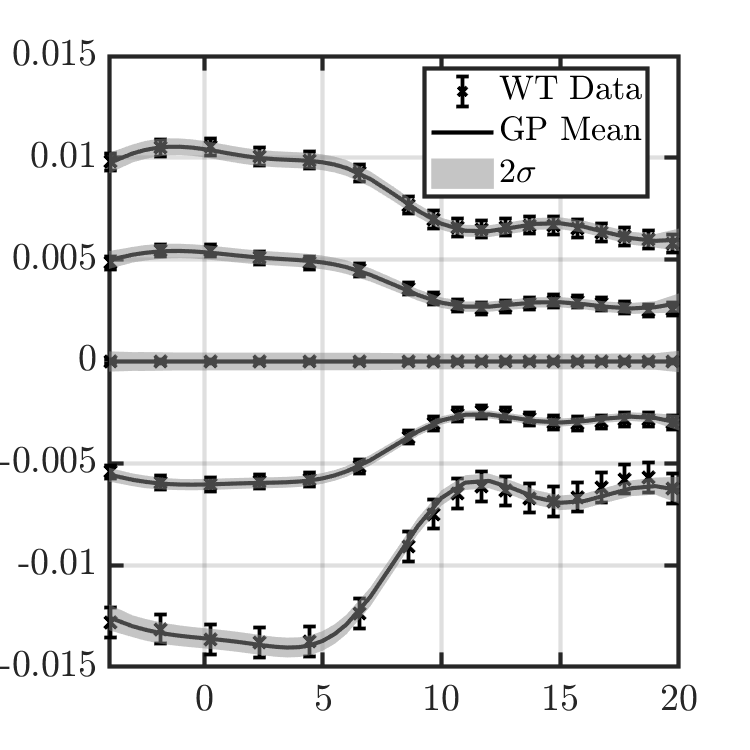
\includegraphics[trim=0 0 0 0, clip, width=.48\textwidth]{code/image_gen/gmatt/1f/wt/images/gps/CRMAIL_beta=4.png} 
    }
    \end{subfigure}
    \hfill
    \begin{subfigure}[\label{subfig:gtt_wt_ctrl_defl}Variation in $\delta_a$ at $\alpha = 8^\circ$ and $\beta=4^\circ$]{
        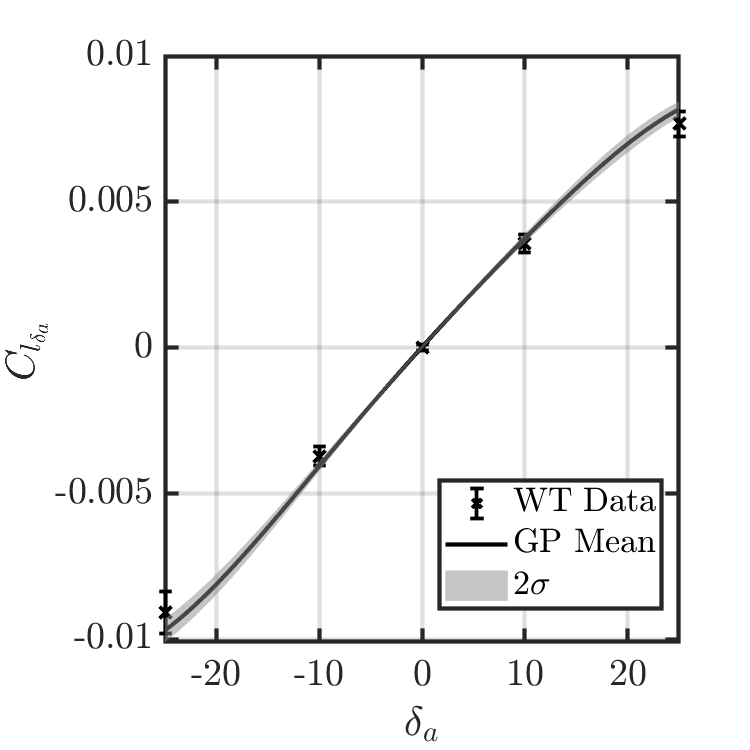
\includegraphics[trim=0 0 0 0, clip, width=.48\textwidth]{code/image_gen/gmatt/1f/wt/images/gps/CRMAIL_alpha=8_beta=4.png} 
    }
    \end{subfigure}
    \caption{Visualization of the 3-Dimensional WT data and resulting single-fidelity GP for the rolling moment due to aileron deflections. \label{fig:gtt_wt_ctrl_gps}}
\end{figure}